
%------------------------------------------------------------------------------
\chapter{Introduction}
\label{chap:intro}
%------------------------------------------------------------------------------

%------------------------------------------------------------------------------
\section{Overview}
\label{sec:overview}
%------------------------------------------------------------------------------

The Sun has been an object of fascination and study for most of humanity's recorded history.
It is the main source of energy and accounts for most of the mass in the solar system.
The history of the Sun began approximately 4.6 billions years ago, with the gravitational collapse of a section of a massive molecular cloud \citep{Bouvier2010}.
This collapse created a protoplanetary disk with a protostar at its centre \citep{Montmerle2006}.
The protostar was composed of hydrogen, helium and lithium, which together accounted for around 98\% of its mass, while the other 2\% were heavier elements formed in younger generations of stars \citep{Zeilik1998}.
For approximately 50 million years after the formation of the protostar, it underwent a slow contraction which increased the temperature and pressure at its core, until it was able to start fusing hydrogen \citep{Yi2001}.
At that point the Sun became a main sequence star, which it will remain for at least another 5 billion years before becoming a red giant \citep{Schroder2008}.
It will subsequently become a red giant, and then a white dwarf, after having ejected nearly half of its mass \citep{Schroder2008}.
The ejected mass will form a planetary nebula, while the white dwarf will survive and may eventually become a hypothetical black dwarf \citep{Bloecker1995}.

The history of solar observations dates back to records of eclipses by Chinese astronomers as early as the year 2000 BCE \citep{Priest2014}.
\emph{Sunspots}, which are areas on the Sun's photosphere that are darker and cooler than their surroundings, have been recorded since at least 800 BCE by the Chinese, and 300 BCE by the ancient Greeks.
The first mention of the \emph{corona}, the high temperature atmosphere of the Sun, is attributed to the Byzantine scholar Leo Diaconus, as he observed the total eclipse of 22 December 968 from Constantinople, although people might have been aware of it as early as the time of Plutarch.
Solar \emph{prominences} were first described in the Russian First Chronicle of Novgorod as ``live embers" coming out of the Sun during the 1 May 1185 eclipse.
For a detailed account of pre-telescope astronomy, see \cite{Hetherington1996}.

\begin{figure}[t]
\centering
\includegraphics[width=\textwidth]{figures/butterfly_diagram.pdf}
\caption{The so-called \emph{butterfly diagram}, displaying the distribution of sunspots across latitudes over time.
Sunspots are most commonly found further from the equator at the beginning of the 11 year cycle, and closer to the equator near its end.
Credit: NASA Marshall Space Flight Center
}
\label{fig:butterfly}
\end{figure}

The advent of modern physics and astronomy led to great advances in solar physics in the past two centuries.
Some of the important discoveries that occurred during the 19\textsuperscript{th} century include the first description of the Sun's spectral lines by Fraunhofer, the discovery of the 11 year sunspot cycle by Schwabe (see Figure \ref{fig:butterfly}), and the first observations of solar flares and spicules by Carrington and Secchi, respectively.
The pace of discovery accelerated during the 20\textsuperscript{th} century, as new instruments, such as the coronagraph, were created, and the theory of \emph{magnetohydrodynamics} (MHD), which is used to describe many solar phenomena, was established.
Other important discoveries include the first description of the solar wind \citep{Parker1958} and the first observations of coronal mass ejections (CMEs).
Finally, our modern view of the Sun has been shaped by the multitude of solar missions that have become operational since the 1990s, such as Yohkoh, TRACE and SDO.
For a more detailed view of recent advances in solar physics, see, for example, \cite{Aschwanden2004, Priest2014}.

%------------------------------------------------------------------------------
\section{Structure and Physical Properties of the Sun}
\label{sec:structure}
%------------------------------------------------------------------------------

The Sun is a highly inhomogeneous nearly perfect sphere of plasma.
Its mean radius has been measured as being $R_\odot = 695.66$ \si{Mm} \citep{Haberreiter2008}, although the International Astronomical Union defines the nominal solar radius as $R_\odot^N = 695.7$ \si{Mm} \citep{Mamajek2015}.
It has a mass of $1.99 \times 10^{30}$ \si{kg} and loses around $1-1.5 \times 10^9$ \si{kg.s^{-1}} due to the solar wind \citep{Parker1958, Priest2014}.
The Sun is composed primarily of hydrogen (over 70\% of the solar mass), and helium (around 27\% of the solar mass), with only trace amounts of other elements, such as oxygen, carbon or nitrogen \citep{Lodders2003}.
The mean distance between the Sun and the Earth is one astronomical unit, defined as 1 \si{au} = \num{149597870700} \si{m}, or approximately $150 \times 10^6$ \si{km} \citep{Capitaine2012}.


In the following Subsections, we shall discuss the structure and physical properties of both the hidden solar interior, and of the visible atmosphere.
According to the latest models, the solar interior consists of four regions: the core, the radiative zone, the tachocline, and the convective zone, listed here from the innermost to the outermost.
The solar atmosphere is composed of the photosphere, chromosphere and corona.
While the solar atmosphere is observable with optical telescopes, due to the high density of solar plasma beneath the photosphere, the solar interior is opaque.
Our current knowledge of the interior is obtained through the mathematical models of helioseismology.

All of the structure described above, as well as some other phenomena that will be discussed later, has been visualised in Figure \ref{fig:sun}.
The majority of the current section has been adapted from \cite{Priest2014}, and should be considered a reference, unless a different reference is stated.

\begin{figure}[t]
\centering
\includegraphics[width=0.99\textwidth]{figures/Sun_structure.png}
\caption{The structure of the Sun. The core, radiative zone, tachocline and convective zone form the opaque inner layers, while the photosphere, chromosphere and corona form the observable atmosphere. Various observable phenomena, including a flare, prominence and photospheric granulation are also presented.
Adapted from Wikipedia.}
\label{fig:sun}
\end{figure}

%------------------------------------------------------------------------------
\subsection{The Solar Interior}
\label{subsec:interior}
%------------------------------------------------------------------------------

The \emph{solar core} extends from the center of the Sun to approximately 0.25 solar radii.
Its temperature is of the order of 15 million \si{K}, and its density around $1.6 \times 10^5$ \si{kg.m^{-3}}, which is enough to enable nuclear fusion.
The core contains approximately half the mass of the Sun in only 1/50 of its volume, and produces 99\% of its energy.
Most of this energy comes from two sets of fusion reactions: the proton-proton chain reaction and the CNO (carbon-nitrogen-oxygen) cycle.
Both of these reactions have the same outcome: four protons (\textsuperscript{1}H) become fused into one helium-4 nucleus (\textsuperscript{4}He), while other atoms only act as catalysts.
As a result of the process of fusion, some of the mass is converted into energy, and escapes in the form of high-energy $\gamma$-rays and also electron neutrinos.

The \emph{radiative zone} is the layer directly above the core, and extends from approximately $0.25 R_\odot$ to $0.7 R_\odot$.
The plasma composing this layer is opaque enough that the mean free path of photons travelling through it is of the order of $10^{-4}$ \si{m}.
If not for this opacity, photons would only take 2 \si{s} to cross the radiative zone, but instead they perform a random walk which lengthens their journey to \num{170000} years.
The numerous collisions that photons experience during this time have a major effect, that of increasing the wavelength of the high-energy $\gamma$-rays emerging from the core, to visible light at the solar surface.

In contrast to the radiative zone where energy is transported via radiative diffusion and thermal conduction, in the \emph{convective zone} the convective instability is the main source of energy transport.
These two sections are separated by a thin shear layer, called the \emph{tachocline} \citep{Spiegel1992}, which is likely significant in the generation of the global solar magnetic field.
The convective zone is the last of the interior layers and extends from around $0.7 R_\odot$ to $1 R_\odot$.

%------------------------------------------------------------------------------
\subsection{The Solar Atmosphere}
\label{subsec:atmosphere}
%------------------------------------------------------------------------------

The solar atmosphere may be divided into four regions which have different physical characteristics (see Figure \ref{fig:sun}).
The lowest of these, the \emph{photosphere}, is the Sun's surface layer and is only around 500 \si{km} thick.
It is where most of the Sun's visible light is emitted.
Most of the photosphere is composed of granules with hot bright centres of rising plasma and cool dark boundaries.
This granulation is caused by turbulent convective motion lifting hot plasma, which subsequently cools and falls, forming the granular boundaries, called intergranular lanes.
Regions of strong magnetic flux may inhibit this convection, and form sunspots.
Granules have diameters ranging from 0.3 to 2 \si{Mm}, and lifetimes of 1 to 20 minutes, with typical values of 5 to 8 minutes \citep{Priest2014}.

The \emph{chromosphere} extends over the photosphere and exhibits various forms of structuring.
The most common of these are spicules, which are dynamic jets that cover the solar surface and form a sort of canopy.

\begin{figure}[h]
\centering
\includegraphics[width=0.8\textwidth]{figures/VAL.png}
\caption{The mean variation of the density and temperature, as described by the VAL  model. Image credit: \cite{Avrett2008}.
}
\label{fig:val}
\end{figure}

The \emph{corona} is the outermost regions of the Sun's atmosphere, separated from the chromosphere by a narrow \emph{transition region}, and extends outwards into the solar wind.
Significant structuring is present in the corona due to the intense magnetic fields that permeate it.
Of particular interest in this Thesis are \emph{coronal loops}.
They are a common form of structuring, comprising of hot plasma (2 to 3 \si{MK}) frozen into the magnetic fields tied to the photosphere.
Coronal loops are waveguides for MHD waves of various modes, an aspect which we examine in Chapter 3 of this Thesis.
Other structures in the corona include coronal holes, X-ray bright points, and coronal streamers.

Coronal mass ejections are large-scale releases of solar plasma from the corona, often following solar flares or prominence eruptions.
Their bulk speeds take a wide range of values, from less than 100 \si{km.s^{-1}} to over 2000 \si{km.s^{-1}}.
They account for approximately 5 to 10 per cent of the solar wind mass-loss.
It is shown in Chapter 2 that the high bulk speed of CMEs makes them particularly prone to the Kelvin-Helmholtz instability.

The mean temperatures and densities of the regions introduced above are commonly described using the VAL (Vernazza-Avrett-Loeset) model \citep{Vernazza1981, Avrett2008}.
According to this model, the density suffers a decrease from approximately $10^{-4}$ \si{kg.m^{-3}} at the base of the photosphere to around $10^{-10}$ \si{kg.m^{-3}} at the transition region, and then falls steeply to almost $10^{-12}$ \si{kg.m^{-3}} in the corona.
The temperature also rises dramatically across the transition region, from a chromospheric value of \num{25000} to over 1 \si{MK} in the corona.
The mechanisms that cause this abrupt increase in temperature are still not well understood, and are a topic of ongoing study.

%------------------------------------------------------------------------------
\section{Equations of Magnetohydrodynamics}
\label{sec:mhdeqns}
%------------------------------------------------------------------------------

In Section \ref{sec:structure} we described some of the main physical properties of the Sun, gave an overview of its large- and small-scale structure, and introduced a number of solar phenomena.
In order to mathematically model this phenomena, we need to employ a suitable framework.
Due to the fact that, in this Thesis, we are mainly concerned with phenomena in the corona, we considered the most appropriate framework the equations of \emph{ideal magnetohydrodynamics} (MHD).

In this Section, we give a brief description of how the ideal MHD equations are obtained, and we motivate their use in modelling coronal phenomena.
The MHD equations may be obtained using two different methods:
\begin{itemize}
\item Averaging the kinetic equations for plasmas;
\item Combining Maxwell's equations for electric and magnetic fields with the fluid equations.
\end{itemize}
The first of these methods is mathematically more complicated and shall be omitted in this section.
However, the relevant derivation may be found in classical works such as \cite{Braginskii1965} or \cite{Chapman1970}, or more modern introductions to MHD, such as \cite{Goossens2003} or \cite{Goedbloed2004}.

For the second, we require the equations of Maxwell, that describe the evolution of the electric field, $\mathbf E(\mathbf{r}, t)$ (measured in \si{V.m^{-1}}), and magnetic field $\mathbf B(\mathbf{r}, t)$ (measured in \si{T}), in response to the current density $\mathbf j(\mathbf{r}, t)$ (measured in \si{A.m^{-2}}) and the total electric charge density $\mathbf \tau(\mathbf{r}, t)$ (measured in \si{C.m^{-3}}).
Additionally, we require the equations of conservation of momentum, mass, and energy, which govern the dynamical evolution of the density, $\rho(\mathbf{r}, t)$ (measured in \si{kg.m^{-3}}), pressure $p(\mathbf{r}, t)$ (measured in \si{N.m^{-2}}), and velocity, $\mathbf{v}(\mathbf{r}, t)$ (measured in \si{m.s^{-1}}), of a fluid.
Here, $\mathbf{r}$ is the position vector, and $t$ is time (measured in \si{s}).

After making a number of simplifying assumptions, we combine these two systems of equations in order to eliminate, $\mathbf{E}, \mathbf{j}$, and $\tau$, and obtain a system of coupled equations in terms of $\mathbf{v}, \mathbf{B}, \rho$, and $p$.

%------------------------------------------------------------------------------
\subsection{Assumptions of Ideal MHD}
\label{subsec:assumpt}
%------------------------------------------------------------------------------

The MHD equations describe the macroscopic dynamics of magnetised plasmas.
As such, we need to establish under what conditions kinetic effects, i.e. small scale effects, stop becoming significant, and the plasma may be treated as a bulk fluid.
This Subsection is based on \cite{Goedbloed2004} and \cite{Priest2014}.

We begin by assuming that the model plasma is \textit{electrically neutral}, which is true for most applications in the solar photosphere and corona.
We define the number densities of positive and negative particles per unit volume, $n_+$ and $n_-$, respectively, and the total number density per unit volume, $n$.
It follows that, for charge neutrality, we require
$
|n_+ - n_-| \ll n.
$
The absence of charge neutrality is called a \textit{charge imbalance}, and such an imbalance produces an electric field with a spatial range of the \textit{Debye length} \citep[see, for example,][]{Boyd2003},
%
\begin{equation}
\label{eq:ass2}
\lambda_D = \sqrt{\frac{\varepsilon_0 k_B T}{n q}}.
\end{equation}
%
The quantities in Equation \eqref{eq:ass2} are defined as follows.
The electric constant, $\varepsilon_0$, also called the permittivity of free space, may be written as
%
\begin{equation}
\label{eq:electricconst}
\varepsilon_0 = \frac{1}{\mu_0 c^2} \approx 8.854187817... \times 10^{-12} \: \si{F.s^{-1}},
\end{equation}
%
where, $\mu_0$ is the magnetic permeability of free space, defined as
%
\begin{equation}
\label{eq:magneticconst}
\mu_0 = 4 \pi \times 10^7 \: \si{N.A^{-2}},
\end{equation}
%
and $c = \num{299792458} \: \si{m.s^{-1}}$ is the speed of light.
$k_B \approx 1.38 \times 10^{-23} \: \si{J.K^{-1}}$ is the Boltzmann constant, and $q$ is the charge of a particle.
We may now define a plasma as a collection of charge particles whose number density, $n$, is very large in a sphere of radius $\lambda_D$,
%
\begin{equation}
\label{eq:debye}
\frac{4}{3} \pi \lambda_D^3 n \gg 1.
\end{equation}
%
Typical values of the Debye length are of the order of $10^{-3}$ \si{m} in the corona, $10^{-11}$ \si{m} in the solar core, and $10$ \si{m} in the solar wind.

The second assumption we must make is that the plasma may be treated as a continuum.
This is valid provided the length-scales of gradients in the plasma are much greater than characteristic plasma lengths, such as the gyroradius (also called the Larmor radius or cyclotron radius), which is defined as
\[
r_g = \frac{m v_\perp}{|q| B}.
\]
Here, $m$ is the mass of the particle, $v_\perp$ is the component of the velocity perpendicular to the magnetic field, and $q$ is the electric charge of the particle.
Furthermore, we assume that the plasma is in thermodynamic equilibrium, such that its distribution function is close to Maxwellian.
This assumption is true for time scales much greater than the collision times, and length scales much greater than the mean free path of the plasma.
The mean free path in the ambient corona may be up to 1 \si{km} due to the low particle density of the plasma.

We also assume that we may treat the plasma as a single fluid.
This is a good approximation for applications to the photosphere and corona, but may not be accurate for models of the chromosphere since interactions between ions and neutrals are significant in that region.

We also assume that the equations are formulated for an inertial frame, and that the typical plasma velocity is non-relativistic.
We may write this second condition as
$
v_0 \ll c,
$
where $v_0$ is the typical speed of the plasma.

Note that, in this Thesis, we only consider adiabatic, inviscid, and ideal plasmas, so that we may neglect any terms related to heat transfer, viscosity and resistivity, when deriving the ideal MHD equations.

Finally, we note that all equations shall be considered in their differential form in \si{m.k.s} units.

%------------------------------------------------------------------------------
\subsection{Maxwell's Equations}
\label{subsec:Max}
%------------------------------------------------------------------------------

We begin by considering the first of Maxwell's equations of classical electrodynamics, which is Gauss's law for the electric field,
%
\begin{equation}
\label{eq:max1}
\nabla \cdot \mathbf E = \dfrac{\tau}{\varepsilon_0}.
\end{equation}
%
This states that the divergence of the electric field is equal to the total electric charge density divided by the electric constant, $\varepsilon_0$, defined in Equation \eqref{eq:electricconst}.

The second equation is the condition that there exist no magnetic monopoles.
This equation is also known as Gauss's law for magnetism, and may be written as
%
\begin{equation}
\label{eq:max2}
\nabla \cdot \mathbf B = 0.
\end{equation}
%
Equation \eqref{eq:max2} states that magnetic fields must be solenoidal vector fields.
As a consequence, point charges of magnetic field, analogous to electric charges, may not exist.

The third equation is the Maxwell-Faraday equation,
%
\begin{equation}
\label{eq:max3}
\nabla \times \mathbf E = - \frac{\partial \mathbf B}{\partial t},
\end{equation}
%
which states that any change of the magnetic field in time, will coincide with a spatially varying non-conservative electric field, and vice-versa.
A straightforward example of this concept is that of the generation of electric current in a dynamo using a permanent magnet, such as a bar magnet.
In such an instrument, a rotating magnet surrounded by coils of wire, creates electric current in the wires.

The final equation is known as Amp\`ere's circuital law,
%
\begin{equation}
\label{eq:max4}
\nabla \times \mathbf B = \mu_0 \mathbf j + \frac{1}{c^2} \frac{\partial \mathbf E}{\partial t},
\end{equation}
%
which states that magnetic fields may be generated through both an induced electric current, and a change in the electric field.
Only the first mechanism was originally included in Amp\`ere's law, while the second mechanism is due to Maxwell.
It follows from Equations \eqref{eq:max3} and \eqref{eq:max4} that time-varying electric and magnetic fields will generate spatially varying magnetic and electric fields, respectively.

%------------------------------------------------------------------------------
\subsection{Equations of Gas Dynamics}
\label{subsec:gas}
%------------------------------------------------------------------------------

Having introduced Maxwell's equations, \eqref{eq:max1} -- \eqref{eq:max4}, we now wish to introduce the equations governing the dynamical evolution of the density, $\rho(\mathbf{r}, t)$, pressure $p(\mathbf{r}, t)$, and velocity $\mathbf{v}(\mathbf{r}, t)$ of a plasma.
Before we proceed, we must introduce the Lagrangian time-derivative of a fluid,
%
\begin{equation}
\label{eq:lagder1}
\frac{\mathrm{D}}{\mathrm{D} t} = \frac{\partial}{\partial t} + \mathbf{v} \cdot \nabla
\end{equation}
%
which is evaluated in the frame of reference of a moving fluid, and differs from the Eulerian time-derivative, $\partial / \partial t$, which is evaluated at a fixed point.

Since we are only concerned with ideal MHD, we only consider the equations of conservation of mass, momentum and energy of adiabatic and inviscid plasmas.
The equation for the evolution of the density, most conveniently written
%
\begin{equation}
\label{eq:mass}
\frac{\mathrm{D} \rho}{\mathrm{D} t} + \rho \nabla \cdot \mathbf{v} = 0,
\end{equation}
%
is called the mass continuity equation, and may also be written
%
\begin{equation}
\label{eq:gas1-1}
\frac{\partial \rho}{\partial t} + \nabla \cdot ( \rho \mathbf{v} ) = 0.
\end{equation}
%
In this form, we can see that it represents conservation of mass, since an increase in density at a point, represented by a positive $\partial \rho / \partial t$, is accompanied by mass flowing in, i.e. $\nabla \cdot ( \rho \mathbf{v} ) < 0$.

We introduce the energy equation, which may be written in terms of the internal energy per unit mass, $e$ (measured in \si{J.kg^{-1}}),
%
\begin{equation}
\label{eq:gas2}
\rho \frac{\mathrm{D} e}{\mathrm{D} t} - \frac{p}{\rho} \frac{\mathrm{D} \rho}{\mathrm{D} t} = - \mathcal{L},
\end{equation}
%
where $\mathcal{L}$ is the energy loss function (measured in \si{J.m^{-3}.s^{-1}}).
Since we are only considering adiabatic processes, the energy gains and losses balance, so that $\mathcal{L} \equiv 0$, and Equation \eqref{eq:gas2} may be written as
%
\begin{equation}
\label{eq:gas2-1}
\rho \frac{\mathrm{D} e}{\mathrm{D} t} - \frac{p}{\rho} \frac{\mathrm{D} \rho}{\mathrm{D} t} = 0,
\end{equation}
%
such that energy is conserved.
In order to further simplify Equation \eqref{eq:gas2-1}, we wish to eliminate the internal energy and obtain an equation relating the pressure and density.
The plasma pressure is determined by an equation of state, which we assume to be the ideal gas law,
%
\begin{equation}
\label{eq:gas2-2}
p = \frac{k_B}{m} \rho T,
\end{equation}
%
where $m$ is the mean mass (measured in \si{kg}) of the particles that make up the plasma, and $T$ is the absolute temperature of the plasma (measured in \si{K}).
For an ideal gas, the heat capacity is constant with temperature, and we may write the internal energy as 
%
\begin{equation}
\label{eq:gas2-3}
e = c_v T,
\end{equation}
%
where $c_v$ is the specific heat at constant volume.
We define the specific heat at constant pressure as
%
\begin{equation}
\label{eq:gas2-4}
c_p = c_v + \frac{k_B}{m},
\end{equation}
%
and the ratio of specific heats (also called the adiabatic index),
%
\begin{equation}
\label{eq:gas2-5}
\gamma = \frac{c_v}{c_p}.
\end{equation}
%
We may write the specific heat at constant volume as
%
\begin{equation}
\label{eq:gas2-6}
c_v = \frac{1}{\gamma - 1} \frac{k_B}{m},
\end{equation}
%
and combine Equations \eqref{eq:gas2-2}, \eqref{eq:gas2-3}, and \eqref{eq:gas2-6} to obtain
%
\begin{equation}
\label{eq:gas2-7}
e = \frac{1}{\gamma - 1} \frac{p}{\rho}.
\end{equation}
%
We substitute \eqref{eq:gas2-7} into \eqref{eq:gas2-1} to obtain the desired form of the energy equation,
%
\begin{equation}
\label{eq:energy}
\frac{\mathrm{D} p}{\mathrm{D} t} - \frac{\gamma p}{\rho} \frac{\mathrm{D} \rho}{\mathrm{D} t} = 0.
\end{equation}
%
It is worth noting that, the adiabatic index is related to the number of degrees of freedom of a molecule by $\gamma = 1 + 2/f$, where $f$ is the number of degrees of freedom.
Since, in this Thesis, we are primarily concerned with fully ionised monoatomic plasmas characteristic of the solar corona, we may assume that $f = 3$, and $\gamma = 5/3$.

The final equation of gas dynamics is the equation of motion for a fluid element, which connects the equations of electrodynamics, described in Subsection \ref{subsec:Max}, with the gas dynamics equations described in the current section.
In order for conservation of momentum to be satisfied, we require
%
\begin{equation}
\label{eq:gas3}
\rho \frac{\mathrm{D} \mathbf v}{\mathrm{D} t} = \mathbf{F},
\end{equation}
%
where $\mathbf{F}$ (measured in units of force density, \si{N.m^{-3}}) is given by
%
\begin{equation}
\label{eq:gas3-1}
\mathbf{F} \equiv - \nabla p + \rho \mathbf{g} + \mathbf{j} \times \mathbf{B} + \tau \mathbf{E}.
\end{equation}
%

%------------------------------------------------------------------------------
\subsection{The Equations of Ideal MHD}
\label{subsec:mhdderiv}
%------------------------------------------------------------------------------

In order to connect the equations of electrodynamics, described in Subsection \ref{subsec:Max}, with the equations of gas dynamics described in Subsection \ref{subsec:gas}, we begin by introducing Ohm's law, which links the electric, magnetic and velocity fields via the current density, such that
%
\begin{equation}
\label{eq:ohm1}
\mathbf{E} + \mathbf{v} \times \mathbf{B} = \eta \mathbf{j},
\end{equation}
%
where $\eta$ is the electrical resistivity (measured in $\si{\Omega.m}$).
In this Thesis, we are not concerned with situations where non-ideal effects, such as resistivity, play an important role.
As such, we may set $\eta = 0$, and Ohm's law reduces to
%
\begin{equation}
\label{eq:ohm2}
\mathbf{E} + \mathbf{v} \times \mathbf{B} = 0.
\end{equation}
%
From Equation \eqref{eq:ohm2}, we see that the typical scales of the magnitude of the electric field, $E$, and magnetic field, $B$, satisfy
%
\begin{equation}
\label{eq:scales1}
E \sim - v B.
\end{equation}
%

We now return to Equation \eqref{eq:max4}, and find that
%
\begin{equation}
\label{eq:scales2}
\frac{1}{c^2} \left| \frac{\partial \mathbf{E}}{\partial t} \right|
\sim \frac{v}{c^2} \frac{B}{t_0}
= \frac{v^2}{c^2} \frac{B}{l_0}
= \mathcal{O}(v^2/c^2),
\end{equation}
%
where $t_0$ and $l_0$ are the characteristic time and length scales.
Here, $\mathcal{O}$, represents the order of a quantity, and is known as Big $\mathcal{O}$ notation.
The quantity in Equation \eqref{eq:scales2} is much smaller than the term on the LHS of Equation \eqref{eq:max4}, which is $|\nabla \times \mathbf{B}| \sim B / l_0$.
It follows that the term in Equation \eqref{eq:scales2} may be neglected from Equation \eqref{eq:max4}, and we recover the original form of Amp\`ere's law,
%
\begin{equation}
\label{eq:ampere}
\mathbf j = \frac{1}{\mu_0} \nabla \times \mathbf B.
\end{equation}
%

The equation of motion, \eqref{eq:gas3}, is also simplified by the assumption of non-relativistic velocities.
Using Equations \eqref{eq:max1} and \eqref{eq:scales1}, we find that the electrostatic acceleration satisfies
%
\begin{equation}
\label{eq:scales3}
\tau |\mathbf{E}| \sim \frac{v B}{\mu_0 c^2 l_0} \times v B
= \frac{v^2}{c^2} \frac{B^2}{\mu_0 l_0}
= \mathcal{O}(v^2/c^2).
\end{equation}
%
Using Equation \eqref{eq:ampere}, we find that $\tau |\mathbf{E}| \ll |\mathbf{j} \times \mathbf{B}| \sim B^2 / \mu_0 l_0$.
This means that the final term in Equation \eqref{eq:gas3-1} may be neglected, and the equation of motion becomes
%
\begin{equation}
\label{eq:momentum}
\rho \frac{\mathrm{D} \mathbf v}{\mathrm{D} t} = - \nabla p + \rho \mathbf{g} + \mathbf{j} \times \mathbf{B},
\end{equation}
%

Finally, we combine Equations \eqref{eq:max3} and \eqref{eq:ohm2} to obtain the induction equation,
%
\begin{equation}
\label{eq:induction}
\frac{\partial \mathbf{B}}{\partial t} - \nabla \times ( \mathbf{v} \times \mathbf{B} ) = 0.
\end{equation}
%
We have, thus, obtained a system of 8 coupled partial differential equations, Equations \eqref{eq:mass}, \eqref{eq:energy}, \eqref{eq:momentum}, and \eqref{eq:induction}, which constitute the system of ideal MHD equations.
Equation \eqref{eq:max2}, the condition that there are no magnetic monopoles, is also part of this system, but is always satisfied if it is satisfied as an initial condition.
We can see this if we take the divergence, $\nabla \cdot$, of Equation \eqref{eq:induction}.

%------------------------------------------------------------------------------
\subsection{Consequences of Ideal MHD}
\label{subsec:conseq}
%------------------------------------------------------------------------------

%The first observation we need to make concerns the conservation of the quantities described by the ideal MHD equations.
%Equations \eqref{eq:mass}, \eqref{eq:energy}, \eqref{eq:momentum}, and \eqref{eq:induction} may be written in such a form that it becomes obvious that mass, energy, momentum, and the magnetic field, respectively, are conserved \citep{Goedbloed2004}.

A first remark on the ideal MHD equations comes from the momentum equation, \eqref{eq:momentum}, where the term $\mathbf{j} \times \mathbf{B}$, called the \textit{Lorentz force}, may be written as
%
\begin{equation}
\label{eq:lorentz}
\mathbf{j} \times \mathbf{B}
= \frac{1}{\mu_0} ( \nabla \times \mathbf B ) \times \mathbf{B}
= \frac{ ( \mathbf{B} \cdot \nabla ) \mathbf{B}}{\mu_0}
- \nabla \left( \frac{\mathbf{B}^2}{2 \mu_0} \right).
\end{equation}
%
The first term on the right-hand side is called the \textit{magnetic tension} force, while the second is the \textit{magnetic pressure} force.
It may be shown that the magnetic tension results in a negative stress in a direction parallel to $\mathbf{B}$, while the magnetic pressure causes a positive stress normal to $\mathbf{B}$ \citep{Goedbloed2004}.

A second result of note is Alfv\'en's frozen flux theorem, which states that, in ideal MHD, magnetic flux is conserved so that the magnetic field moves with the plasma.
This is in addition to the quantities that we already know are conserved, from the Euler equations, namely mass, energy and momentum.

While the ideal MHD equations have various other properties, we restrict our discussion to the two above, as they are most relevant in this Thesis.


%------------------------------------------------------------------------------
\subsection{The Linear Ideal MHD Equations}
\label{subsec:linearmhd}
%------------------------------------------------------------------------------

The nonlinear form of the MHD Equations is difficult to treat analytically in most situations.
For many applications, we may \textit{linearise} Equations \eqref{eq:mass}, \eqref{eq:energy}, \eqref{eq:momentum}, and \eqref{eq:induction} in the following way.
We assume that the dependent variables, $\mathbf{v}, \mathbf{B}, \rho$ and $p$, may be split into two distinct quantities: a \textit{background} (or \textit{equilibrium}) value, and a small \textit{perturbation}.
We write this as
%
\begin{align}
\begin{split}
\label{eq:perturbations}
\mathbf{v} & = \mathbf{v_0} + \mathbf{v'},
\qquad
\mathbf{B} = \mathbf{B_0} + \mathbf{b'},
\\
\rho & = \rho_0 + \rho',
\qquad
p = p_0 + p',
\end{split}
\end{align}
%
where the subscript $0$ represents the background value, and the apostrophe denotes the perturbation.
We assume that the perturbations of the magnetic field, density and pressure are much smaller than their equilibrium values, i.e.
%
\begin{equation}
| \mathbf{B_0} | \gg | \mathbf{b'} |,
\qquad
\rho_0 \gg \rho',
\qquad
p_0 \gg p'.
\end{equation}
%
This assumption is not always applicable to the velocity perturbation since the background flow may be zero ($\mathbf{v_0} = \mathbf 0$).
In such cases, we say that the velocity perturbation is much smaller than some other characteristic speed of the system, such as the local speed of sound,
%
\begin{equation}
\label{eq:soundspeed}
c_s = \sqrt{ \gamma \frac{p_0}{\rho_0} },
\end{equation}
%
or Alfv\'en speed
%
\begin{equation}
\label{eq:alfvenspeed}
v_A = \sqrt{ \frac{B_0^2}{\mu_0 \rho} }.
\end{equation}
%
It is worth noting that the background quantities may be inhomogeneous spatially and may evolve temporally.

We, now, insert Equations \eqref{eq:perturbations} into Equations \eqref{eq:mass}, \eqref{eq:energy}, \eqref{eq:momentum}, and \eqref{eq:induction}, and neglect nonlinear coupling due to products of perturbations.
This yields the system of linear ideal MHD equations
%
\begin{align}
\label{eq:masslin}
& \frac{\mathrm{D} \rho'}{\mathrm{D} t}
+ \rho_0 \nabla \cdot \mathbf{v'}
= 0,
\\[0.2cm]
\label{eq:enerlin}
& \frac{\mathrm{D} p'}{\mathrm{D} t}
= c_s^2 \frac{\mathrm{D} \rho'}{\mathrm{D} t},
\\[0.2cm]
\label{eq:momlin}
\rho_0 & \frac{\mathrm{D} \mathbf v'}{\mathrm{D} t}
= - \nabla p'
+ \frac{1}{\mu_0} (\nabla \times \mathbf{b'}) \times \mathbf{B_0},
\\[0.2cm]
\label{eq:indlin}
& \frac{\partial \mathbf{b'}}{\partial t}
= \nabla \times (\mathbf{v_0} \times \mathbf{b'})
+ \nabla \times (\mathbf{v'} \times \mathbf{B_0}),
\\[0.2cm]
\nonumber
& \nabla \cdot \mathbf{b}' = 0,
\end{align}
%
where the Lagrangian derivative is now defined as
%
\begin{equation}
\label{eq:lagder2}
\frac{\mathrm{D}}{\mathrm{D} t}
= \frac{\partial}{\partial t}
+ \mathbf{v_0} \cdot \nabla,
\end{equation}
%
and the apostrophe was dropped when writing the perturbations.
In deriving Equations \eqref{eq:masslin} - \eqref{eq:indlin}, we have neglected gravity, since the models we derive in this Thesis have applications to small-scale phenomena, where gravity does not have a strong effect.
We also assumed that $\mathbf{B_0}, \rho_0$ and $p_0$ are spatially homogeneous in each layer, and do not evolve temporally (i.e. independent of $\mathbf{r}$ and $t$), and $\mathbf{v_0}$ is homogeneous in space in each layer (i.e. independent of $\mathbf{r}$).
These assumptions are not true in general, but are sufficient for the analyses in this Thesis.

%------------------------------------------------------------------------------
\subsection{Equations of Incompressible Ideal MHD}
\label{subsec:inc-mhd}
%------------------------------------------------------------------------------

A special form of the ideal MHD equations, which we will make use of later in this Thesis, assumes that all motion is incompressible.
We define incompressibility as the property that density is constant in a fluid, such that the MHD Equations (neglecting gravity) are reduced to
%
\begin{align}
\label{eq:mominc}
\frac{\mathrm{D} \mathbf v}{\mathrm{D} t}
& = - \frac{1}{\rho} \nabla p_T
+ \frac{1}{\mu_0 \rho} ( \mathbf{B} \cdot \nabla ) \mathbf{B},
\\[0.2cm]
\label{eq:indinc}
\frac{\mathrm{D} \mathbf B}{\mathrm{D} t}
& = ( \mathbf{B} \cdot \nabla ) \mathbf{v},
\\[0.2cm]
\label{eq:divv}
\nabla \cdot \mathbf{v} & = 0,
\\[0.1cm]
\nonumber
\nabla \cdot \mathbf{B} & = 0,
\end{align}
%
where $p_T$ is the total (gas plus magnetic) pressure, and the Lagrangian derivative is given by Equation \eqref{eq:lagder1}.

Following the method described in Subsection \ref{subsec:linearmhd}, we linearise Equations \eqref{eq:mominc} - \eqref{eq:divv}, and obtain
%
\begin{align}
\label{eq:mominclin}
\frac{\mathrm{D} \mathbf v'}{\mathrm{D} t}
& = - \frac{1}{\rho_0} \nabla p_T'
+ \frac{1}{\mu_0 \rho_0} ( \mathbf{B_0} \cdot \nabla ) \mathbf{b'},
\\[0.2cm]
\label{eq:indinclin}
\frac{\mathrm{D} \mathbf b'}{\mathrm{D} t}
& = ( \mathbf{B_0} \cdot \nabla ) \mathbf{v'},
\\[0.2cm]
\label{eq:divvlin}
\nabla \cdot \mathbf{v'} & = 0,
\\[0.1cm]
\nonumber
\nabla \cdot \mathbf{b}' & = 0,
\end{align}
%
where $p_T'$ is the perturbation of the total pressure, and the Lagrangian derivative is given by Equation \eqref{eq:lagder2}.
As in Subsection \ref{subsec:linearmhd}, we have assumed that the background quantities are spatially homogeneous, and $\mathbf{B_0}$ is also independent of $t$.

We now introduce the plasma displacement, $\bm \xi (\mathbf{r}, t)$, which is related to the velocity by
%
\begin{equation}
\label{eq:xi}
\mathbf{v'}
= \frac{\mathrm{D} \bm \xi}{\mathrm{D} t}
= \frac{\partial}{\partial t}
+ ( \mathbf{v_0} \cdot \nabla ) \bm \xi.
\end{equation}
%
Substituting Equation \eqref{eq:xi} into Equation \eqref{eq:divvlin}, we obtain
%
\begin{equation}
\frac{\mathrm{D}}{\mathrm{D} t} ( \nabla \cdot \bm \xi ) = 0,
\end{equation}
%
since $\mathbf{v_0}$ is independent of $\mathbf{r}$, meaning that the operators $\mathrm{D}/\mathrm{D} t$ and $\nabla \cdot$ commute.
The Lagrangian derivative cannot be zero since $\bm \xi$ is time-dependent, which implies that the displacement must also be divergence free, i.e.
%
\begin{equation}
\label{eq:divxi}
\nabla \cdot \bm \xi = 0.
\end{equation}
%
We will use Equation \eqref{eq:divxi} in Chapter 3.

%------------------------------------------------------------------------------
\section{Magnetohydrodynamic Waves}
\label{sec:mhdwaves}
%------------------------------------------------------------------------------

A fundamental property of the system of linear MHD equations presented in Subsection \ref{subsec:linearmhd} is that it allows for solutions in the form of waves.
In the following Subsections, we shall give a brief analysis of wave motions in both homogeneous media, and in the presence of structuring.
In this Thesis, we are primarily concerned with magnetoacoustic waves, and although Alfv\'en waves are mentioned, they will not receive a detailed description.

In Subsection \ref{subsec:linearmhdwaves}, we derive the dispersion equation for the basic wave modes that may propagate in a homogeneous unbounded plasma governed by the ideal linear MHD equations.
In the rest of the Section, we discuss the behaviour of the magnetoacoustic modes in the presence of three types of structuring: a plane Cartesian \emph{interface} separating two media, two parallel interfaces which form a \emph{slab}, and the \emph{cylindrical flux tube}.

Our discussion of the magnetoacoustic modes in structured plasmas is largely based on the derivations included in \cite{Roberts1981, Roberts1981b, Edwin1982}, as well as \cite{Goedbloed2004, Priest2014}.
It is worth noting, though, that the study of magnetoacoustic waves in structured media has a longer history, with works such as \cite{Cram1975, Defouw1976, Roberts1978, Wilson1978, Roberts1979, Wentzel1979, Wilson1979, Spruit1981} having set the foundations for the more structured approach of Roberts and Edwin.

%------------------------------------------------------------------------------
\subsection{Linear MHD Waves in a Homogeneous Medium}
\label{subsec:linearmhdwaves}
%------------------------------------------------------------------------------

We begin by assuming that all background quantities are homogeneous, i.e. independent of $\mathbf{r}$ and $t$. 
Furthermore, we assume that the background medium is static ($\mathbf{v_0} = \mathbf 0$), and the magnetic field is defined as $\mathbf{B_0} = (0, 0, B_0)$, without loss of generality.
The assumption that $\mathbf{v_0} = \mathbf 0$ is made in order to discuss only MHD waves, and not flow instabilities.
The MHD Equations \eqref{eq:masslin} - \eqref{eq:indlin} may, therefore, be reduced to
%
\begin{align}
\label{eq:enerlin2}
& \frac{\partial p'}{\partial t}
= - c_s^2 \rho_0 \nabla \cdot \mathbf{v'},
\\[0.2cm]
\label{eq:momlin2}
\rho_0 & \frac{\partial \mathbf v'}{\partial t}
= - \nabla p'
+ \frac{1}{\mu_0} (\nabla \times \mathbf{b'}) \times \mathbf{B_0},
\\[0.2cm]
\label{eq:indlin2}
& \frac{\partial \mathbf{b'}}{\partial t}
= \nabla \times (\mathbf{v'} \times \mathbf{B_0}),
\\[0.2cm]
\nonumber
& \nabla \cdot \mathbf{b}' = 0.
\end{align}
%
where we have combined the mass and energy equations.
Once again, we make use of the displacement vector, first introduced in Equation \eqref{eq:xi}.
Since we have assumed no background flow, the displacement is now related to the velocity as
%
\begin{equation}
\label{eq:xihom}
\mathbf{v'}
= \frac{\partial \bm \xi}{\partial t}.
\end{equation}
%
We introduce Equation \eqref{eq:xihom} into Equations \eqref{eq:enerlin2} and \eqref{eq:indlin2}, and we may immediately integrate them with respect to time to obtain
%
\begin{align}
\label{eq:enerlin3}
& p'
= - c_s^2 \rho_0 \nabla \cdot \bm \xi,
\\[0.2cm]
\label{eq:indlin3}
& \mathbf{b'}
= \nabla \times (\bm \xi \times \mathbf{B_0}).
\end{align}
%
Substituting Equations \eqref{eq:xihom}, \eqref{eq:enerlin3}, and \eqref{eq:indlin3} into \eqref{eq:momlin2} yields
%
\begin{equation}
\label{eq:goveqhom}
\frac{\partial^2 \bm \xi}{\partial t^2}
= c_s^2 \nabla (\nabla \cdot \bm \xi)
+ \frac{1}{\mu_0 \rho_0} \mathbf{B_0} \times ( \nabla \times \nabla \times (\mathbf{B_0} \times \bm \xi ))
\end{equation}
%
In deriving Equation \eqref{eq:goveqhom}, we have used the property that the cross product is anti-commutative.

We consider plane wave solutions of the form
%
\begin{equation}
\label{eq:xiplane}
\bm \xi = \bm{\hat \xi} \mathrm{e}^{i (\mathbf{k} \cdot \mathbf{r} - \omega t)},
\end{equation}
%
where $\mathbf{k} = (k_x, 0, k_z)$ is the wave vector, and $\omega$ is the angular frequency.
The $\bot$ and $\parallel$ signs represent the components of the wave vector perpendicular and parallel to the magnetic field, respectively.
The differential operators now turn into algebraic multiplication factors,
%
\begin{equation}
\nabla \to i \mathbf{k}, \qquad \frac{\partial}{\partial t} \to - i \omega,
\end{equation}
%
and Equation \eqref{eq:goveqhom} becomes
%
\begin{equation}
\label{eq:goveqhom2}
- \omega^2 \bm{\hat \xi}
= c_s^2 \mathbf{k} (\mathbf{k} \cdot \bm{\hat \xi})
+ \frac{1}{\mu_0 \rho_0} \mathbf{B_0} \times ( \mathbf{k} \times \mathbf{k} \times (\mathbf{B_0} \times \bm{\hat \xi} )).
\end{equation}
%
We now introduce the vectorial Alfv\'en speed,
%
\begin{equation}
\label{eq:valfven}
\mathbf{v_A} = \frac{\mathbf{B_0}}{\sqrt{\mu_0 \rho_0}}
= (0, 0, v_A),
\end{equation}
%
and, with the help of the vector identities in \cite{Goedbloed2004}, we rewrite Equation \eqref{eq:goveqhom2} as
%
\begin{equation}
\label{eq:goveqhom3}
\left\{
\left[ \omega^2 - (\mathbf{k} \cdot \mathbf{v_A})^2 \right] \mathbf{I}
- (c_s^2 + v_A^2) \mathbf{k} \mathbf{k}
+ \mathbf{k} \cdot \mathbf{v_A} (\mathbf{k} \mathbf{v_A} + \mathbf{v_A} \mathbf{k})
\right\}
\cdot \bm{\hat \xi} = 0,
\end{equation}
%
where $\mathbf{I}$ is the unit tensor, and the lack of symbols between vectors, as in $\mathbf{k}\mathbf{k}$, represents the dyadic product.
Equation \eqref{eq:goveqhom3} may be written in matrix form as
%
\begin{equation}
\label{eq:goveqhom4}
\begin{pmatrix}
\omega^2 - k_x^2 (c_s^2 + v_A^2) - k_z^2 v_A^2 & 0 & - k_x k_z c_s^2
\\
0 & \omega^2 - k_z^2 v_A^2 & 0
\\
- k_x k_z c_s^2 & 0 & \omega^2 - k_z^2 c_s^2
\end{pmatrix}
\begin{pmatrix}
\hat \xi_x
\\
\hat \xi_y
\\
\hat \xi_z
\end{pmatrix}
=
\mathbf{0}.
\end{equation}
%
In order for Equation \eqref{eq:goveqhom3} to have non-trivial solutions, we require that the determinant of the matrix in Equation \eqref{eq:goveqhom4} be zero.
We calculate the determinant and obtain the dispersion relation for MHD waves in a homogeneous unbounded medium,
%
\begin{equation}
\label{eq:disprelhom}
(\omega^2 - k_z^2 v_A^2)
\big[
\omega^4 - \omega^2 k^2 (c_s^2 + v_A^2)
+ k_z^2 k^2 v_A^2 c_s^2
\big]
= 0,
\end{equation}
%
where $k = |\mathbf{k}| = \sqrt{k_x^2 + k_z^2}$.

Before we analyse Equation \eqref{eq:disprelhom}, we note that, due to the fact that we obtained the dispersion relation from a description of the system in terms of the displacement, we omitted the entropy wave.
This mode, corresponding to $\omega = 0$, is degenerate in the sense that it involves no perturbations of the flow, magnetic field or pressure.
It constitutes a perturbation of the entropy of the system (density and internal energy) which would propagate if a background flow was present.

The first class of solutions of Equation \eqref{eq:disprelhom} are obtained from the quadratic factor, and are called \textit{Alfv\'en waves}.
They propagate with frequency
%
\begin{equation}
\label{eq:alfvenhom}
\omega = \pm \omega_A = \pm k_z v_A = \pm k v_A \cos \phi,
\end{equation}
%
where $\phi$ is the angle between $\mathbf{k}$ and $\mathbf{B_0}$, and $\omega_A$ is called the Alfv\'en frequency.
The $\pm$ represents the two possible solutions: one propagating in the direction of $\mathbf{B_0}$, and corresponding to the $+$ sign, and the other propagating in the opposite direction, and corresponding to the $-$ sign.
These waves are incompressible and purely transverse.

The second category of solutions of Equation \eqref{eq:disprelhom} we discuss are \textit{magnetoacoustic} (or \textit{magnetosonic}) \textit{waves}, which are obtained from the quartic factor.
They are split into two categories, slow modes and fast modes, which propagate with frequencies
%
\begin{equation}
\label{eq:slowfast1}
\omega = \pm \omega_s, \qquad \omega = \pm \omega_f,
\end{equation}
%
respectively.
The slow and fast frequencies are defined as
%
\begin{equation}
\label{eq:slowfast2}
\omega_{s, f} = \frac{1}{2} k^2 (c_s^2 + v_A^2)
\big( 1 \pm \sqrt{1 - 4 c_T^2 \cos^2 \phi} \big),
\end{equation}
%
where
%
\begin{equation}
\label{eq:tubespeed}
c_T = \frac{c_s v_A}{\sqrt{c_s^2 + v_A^2}},
\end{equation}
%
is called the tube speed (or cusp speed or slow speed).
Similarly to the Alfv\'en wave solutions, the $\pm$ sign in Equation \eqref{eq:slowfast1} corresponds to forward $(+)$ and backward $(-)$ propagating waves.
The $\pm$ sign in Equation \eqref{eq:slowfast2} corresponds to either the fast mode $(+)$, or the slow mode $(-)$.

%------------------------------------------------------------------------------
\subsection{Linear MHD Waves at a Tangential Interface}
\label{subsec:linearmhdint}
%------------------------------------------------------------------------------

For the first case of inhomogeneous structuring, we utilise a Cartesian coordinate system as in the previous section, and introduce a tangential discontinuity in the $yz$-plane at $x=0$.
This interface separates regions of different homogeneous plasma density, temperature, pressure and magnetic field.
We use the subscript $0$ and $1$ to denote background quantities for $x<0$ and $x>0$, respectively.
The background magnetic field is assumed to be parallel to the $z$-axis on both sides of the interface.

Since the described system is inhomogeneous along the $x$-axis, we may no longer Fourier decompose the MHD Equations \eqref{eq:masslin} - \eqref{eq:indlin}, with respect to $x$.
Furthermore, we only wish to study magnetoacoustic waves propagating along the interface, which we accomplish by assuming that all variables are independent of $y$.
This implies a decomposition of the form $f(\mathbf{r}, t) = \hat f(x) \exp{i(k_z z - \omega t)}$, where $f$ stands for any of the dependent variables.
We also drop the apostrophe from the perturbed quantities for ease of writing.

Our aim is to obtain governing equations for both sides of the interface, solve them, and match the solutions across the interface using appropriate boundary conditions.
We save the derivation of the governing equations for Chapter 2, and present the equation directly,
%
\begin{equation}
\label{eq:goveqinterface}
\frac{\mathrm{d}^2 \hat{v}_x}{\mathrm{d} x^2} - m_{j}^2 \hat{v}_x = 0,
\end{equation}
%
where
%
\begin{equation}
\label{eq:m0}
m_j^2 = k_z^2 
\frac{(c_j^2 - c_{ph}^2)(v_{A j}^2 - c_{ph}^2)}
{(c_j^2 - v_{A j}^2)(c_{T j}^2 - c_{ph}^2)},
\qquad
j = 0, 1.
\end{equation}
%
Here, $\hat{v}_x$ is the component of the velocity perturbation perpendicular to the boundary, $c_j$ are the sound speeds, $v_{A j}$ are the Alfv\'en speeds, $c_{T j}$ are the tube speeds, and $c_{ph} = \omega / k_z$ is the phase speed.
The parameter $m_j$ is sometimes called the effective wavenumber.
Note that the derivation for Equations \eqref{eq:goveqinterface} and \eqref{eq:m0} may also be found in \cite{Roberts1981}, or in modern textbooks such as \cite{Goedbloed2004} or \cite{Priest2014}.

Equation \eqref{eq:goveqinterface} has two distinct classes of solutions: \emph{trapped modes}, with $m_j^2 > 0$, which decay as $x \to \infty$ (see Figure \ref{fig:waves}a), and \emph{leaky modes}, with $m_j^2 < 0$, which propagate towards infinity.
We also note that there exists an unbound state propagating from infinity.
We only consider trapped modes and solve Equation \eqref{eq:goveqinterface},
%
\begin{equation}
\label{eq:vxinterface}
\hat{v}_x (x) = 
\begin{cases}
C_0 \mathrm{e}^{m_0 x}, & x < 0,
\\
C_1 \mathrm{e}^{- m_1 x}, & x > 0,
\end{cases}
\end{equation}
%
where $C_0$ and $C_1$ are arbitrary constants.
The boundary conditions imposed at $x=0$ are that of \emph{continuity of displacement}, and \emph{continuity of total pressure}.
Since we are considering a static background $(\mathbf{v_0} = \mathbf{0})$, the first of these conditions is equivalent to continuity of $\hat{v}_x$.
The total pressure is found to be
%
\begin{equation}
\label{eq:pT}
\hat p_T = \frac{i \rho_j}{\omega} (c_j^2 + v_{A j}^2) \frac{c_{T j}^2 - c_{ph}^2}{c_j^2 - c_{ph}^2} \frac{\mathrm{d} \hat{v}_x}{\mathrm{d} x},
\end{equation}
%
and the condition of continuity of total pressure yields the dispersion relation for waves propagating along an interface,
%
\begin{equation}
\label{eq:disprelint}
c_{ph}^2 = v_{A 0}^2 - \frac{\rho_1 m_0}{\rho_1 m_0 + \rho_0 m_1} ( v_{A 0}^2 - v_{A 1}^2 ).
\end{equation}
%

\begin{figure}[t]
\centering
\includegraphics[width=\textwidth]{figures/waves.pdf}
\caption{A schematic representation of the profile of the velocity amplitude for three different cases: (a) trapped waves on an interface; (b) surface waves in a slab; (c) body waves in a slab. Adapted from \cite{Priest2014}.
}
\label{fig:waves}
\end{figure}

%------------------------------------------------------------------------------
\subsection{Linear MHD Waves on a Slab in a Symmetric Environment}
\label{subsec:linearmhdslab}
%------------------------------------------------------------------------------

The \emph{magnetic slab}, formed of two parallel interfaces in a non-magnetic environment, was considered by \cite{Roberts1981b}, and in a magnetic environment by \cite{Edwin1982}.
Here, we consider a slab with boundaries at $\pm x_0$ in a non-magnetised symmetric environment.
Background quantities will be denoted by subscripts $0$ and $1$ in the regions $|x| < x_0$ and $|x| > x_0$, respectively.
Equation \eqref{eq:goveqinterface} now has trapped solutions of the form
%
\begin{equation}
\label{eq:vxslab}
\hat{v}_x (x) = 
\begin{cases}
C_{10} \mathrm{e}^{m_1 (x + x_0)}, & x < - x_0,
\\
C_{00} \cosh m_0 x + C_{01} \sinh m_0 x, & |x| \leq x_0,
\\
C_{11} \mathrm{e}^{-m_1 (x - x_0)}, & x > x_0,
\end{cases}
\end{equation}
%
where $C_{00}, C_{01}, C_{10}, C_{11}$ are constants.
The sign of $m_0^2$ determines the nature of the waves within the slab.
If $m_0^2 > 0$, the wave is evanescent inside the slab and is called a \emph{surface} mode (Figure \ref{fig:waves}b), whereas if $m_0^2 < 0$, the wave is oscillatory inside the slab and is called a \emph{body} mode (Figure \ref{fig:waves}c).
Furthermore, if $C_{00} = 0$, then $\hat{v}_x (x)$ is an odd function, while if $C_{01} = 0$, then $\hat{v}_x$ is an even function.

\begin{figure}[t]
\centering
\includegraphics[width=\textwidth]{figures/saus_kink.pdf}
\caption{A schematic representation of the two modes of oscillation of a magnetic slab.
}
\label{fig:modessym}
\end{figure}

The total pressure defined in \eqref{eq:pT} is used, and we apply the boundary conditions as for the interface to obtain the dispersion relation for waves propagating along a magnetic slab embedded in a symmetric magnetic environment.
The dispersion relation is factorised into two separate equations,
%
\begin{align}
\begin{split}
\label{eq:disprelslab}
\rho_1 (v_{A 1}^2 - c_{ph}^2) m_0 \tanh (m_0 x_0)
+ \rho_0 (v_{A 0}^2 - c_{ph}^2) m_1 = 0,
\\[0.3cm]
\rho_1 (v_{A 1}^2 - c_{ph}^2) m_0 \coth (m_0 x_0)
+ \rho_0 (v_{A 0}^2 - c_{ph}^2) m_1 = 0,
\end{split}
\end{align}
%
where the equation containing $\tanh$/$\coth$ corresponds to the $\sinh$/$\cosh$ term in Equation \eqref{eq:vxslab}.
It follows that the $\tanh$ and $\coth$ equations describe modes of oscillation whose displacements are antisymmetric and symmetric around $x=0$, respectively.
These modes are called the \emph{sausage} and \emph{kink} modes, and are illustrated in Figure \ref{fig:modessym}.
Approximate analytical solutions, as well as general numerical solutions to Equations \eqref{eq:disprelslab} may be found, for example in \cite{Edwin1982}.

Solutions of Equations \eqref{eq:disprelslab} are always neutrally stable since $\omega^2 > 0$.
If $\omega^2 < 0$, the left hand side of Equations \eqref{eq:disprelslab} would always be positive, and we would have a contradiction.
Therefore, $\omega$ is real, and $\exp{i(k_z z - \omega t)}$ is always oscillatory.
This also makes sense from a physical point of view since there are no effects that may cause the equilibrium to become unstable, such as gravity or shearing flows.
We shall encounter dispersion relations with complex solutions in Chapter 2.

%------------------------------------------------------------------------------
\subsection{Linear MHD Waves in a Cylindrical Flux Tube}
\label{subsec:linearmhdcyl}
%------------------------------------------------------------------------------

The final type of structuring that we need to address is the cylindrical flux tube.
We now use the cylindrical coordinate system $(r, \phi, z)$ and assume that a cylindrical interface at $r = r_0$ separates an interior region, denoted with the subscript $0$, from an exterior region, denoted by the subscript $1$.

Similarly to Subsections \ref{subsec:linearmhdint} and \ref{subsec:linearmhdslab}, we write perturbations of the cylindrical interface as $f = \hat{f} \exp\{i (k_z z + m \phi - \omega t)\}$, where $k_z$ and $\phi$ are the wavenumbers corresponding to the $z$- and $\phi$-directions, respectively.
The linear ideal MHD equations may now be reduced to the governing equation
%
\begin{equation}
\label{eq:goveqcyl}
\frac{\mathrm{d}^2 \hat p_T}{\mathrm{\mathrm{d} t^2}}
+ \frac{1}{r} \frac{\mathrm{d} \hat p_T}{\mathrm{d} r}
+ \left( \frac{m^2}{r^2} + m_j^2 \right) \hat p_T = 0,
\end{equation}
%
where $m_j$ is defined in Equation \eqref{eq:m0}, the total pressure is related to the radial component of the velocity as
%
\begin{equation}
\label{eq:ptvr}
\frac{\mathrm{d} \hat p_T}{\mathrm{d} r} = - i \omega \rho_0 (\omega^2 - k_z^2 v_A^2) \hat v_r,
\end{equation}
%
and $m$ is an integer.
The full derivation of Equations \eqref{eq:goveqcyl} and \eqref{eq:ptvr} are not included in this Thesis, and may be found in \cite{Edwin1983}, or more recent works such as \cite{Goedbloed2004, Priest2014}.

The solutions to Equation \eqref{eq:goveqcyl} in the interior region ($r < r_0$) that are bounded on the axis of the cylinder, i.e. at $r = 0$, have the form
%
\begin{equation}
\label{eq:pti}
\hat p_T = C_0
\begin{cases}
I_m (m_0 r), & m_0^2 > 0,
\\
J_m (m_0 r), & n_0^2 = - m_0^2 > 0,
\end{cases}
\end{equation}
%
where $C_0$ is an arbitrary constant, and $J_m$ and $I_m$ are the Bessel function of the first kind of order $m$ and modified Bessel function of the first kind of order $m$, respectively.
The solution of Equation \eqref{eq:goveqcyl} in the exterior region ($r > r_0$) which is evanescent as $r \to \infty$ is
%
\begin{equation}
\label{eq:pte}
\hat p_T = C_1 K_m (m_1 r),
\end{equation}
%
where $C_1$ is an arbitrary constant and $K_m$ is the modified Bessel function of the second kind.
Here $m_0$ and $m_1$ are defined as in Equation \eqref{eq:m0}.

Using the boundary conditions of continuity of radial velocity and continuity of total pressure, we obtain the dispersion relation for surface modes
%
\begin{equation}
\label{eq:disprelcyl}
\rho_0 (v_{A i}^2 - c_{ph}^2) m_1 \frac{K_m'(m_1 r_0)}{K_m(m_1 r_0)}
= \rho_1 (v_{A e}^2 - c_{ph}^2) m_0 \frac{I_m'(m_0 r_0)}{I_m(m_0 r_0)},
\end{equation}
%
where the dash represents the first derivative with respect to the argument.
For body modes, the Bessel function $I_m$ is replaced by $J_m$, and the effective wavenumber $m_0$ is replaced by $n_0$, where $n_0^2 = - m_0^2$.

\begin{figure}[t]
\centering
\includegraphics[width=0.8\textwidth]{figures/modes_cyl.pdf}
\caption{A schematic representation of a cut-through of a cylindrical flux tube undergoing a sausage oscillation ($m=0$), kink oscillation ($m=1$), and an $m=4$ fluting oscillation. Adapted from \cite{Murdin2001}.
}
\label{fig:modescyl}
\end{figure}

Much like Equations \eqref{eq:disprelslab}, Equation \eqref{eq:disprelcyl} only has stable solutions ($\omega^2 > 0$).
The main difference between the solutions of the dispersion relation of waves propagating along a slab and that of waves propagating along a cylinder, is that the cylindrical geometry supports additional modes of oscillation.
The parameter $m$ determines the wave mode, with $m=0$ and $m=1$ being the familiar sausage and kink modes, and $m>1$ corresponding to the \emph{fluting} modes (see Figure \ref{fig:modescyl}).

In deriving Equation \eqref{eq:disprelcyl} we assumed that the magnetic field is vertically straight both within and outside of the tube, which does not necessarily hold in applications to solar cylindrical magnetic waveguides.
Several models of cylindrical flux tubes with twisted magnetic fields have been devised by, for example, \cite{Bennett1999, Erdelyi2006, Erdelyi2007, Ruderman2007, Erdelyi2010, Vasheghani2010, Ruderman2015a, Ruderman2015b}.
These shall be important in the context of the Kelvin-Helmholtz instability of transversely (kink) oscillating flux tubes, in Chapter 3.

%------------------------------------------------------------------------------
\subsection{Coronal Loop Oscillations}
\label{subsec:loops}
%------------------------------------------------------------------------------

In Subsections \ref{subsec:linearmhdint} - \ref{subsec:linearmhdcyl} we derived three of the most common theoretical models for magnetoacoustic waves in structured media relevant for solar applications.
In this Subsection we wish to apply some of the theory discussed previously to one of the most fascinating objects of research in solar physics: coronal loops, first introduced in Subsection \ref{subsec:atmosphere}, and their modes of oscillation.

Coronal loops are most often modelled as straight magnetic cylinders, due to the fact that the curvature of the loop often plays little role on the properties of the oscillations \citep{TVD2004}.
It follows that the loops would exhibit the modes of oscillation described in Subsection \ref{subsec:linearmhdcyl}.
Interpreting the observed modes in terms of the cylindrical model, as well as other models which we shall not discuss here, has led to the creation of the field of coronal seismology.
It uses the properties of observed waves, in addition to knowledge of some background quantities, in order to determine parameters that are difficult to measure, such as the strength of the magnetic field.

While observations of sausage waves in coronal loops do exist \citep{Nakariakov2003, Srivastava2008}, by far the most common mode of oscillation is the fast kink mode.
For reviews on the subject, see, for example, \cite{Nakariakov2005, Ruderman2009, DeMoortel2012}.

\begin{figure}[t]
\centering
\includegraphics[width=0.8\textwidth]{figures/time_distance.png}
\caption{The temporal evolution of the displacement of the loop studied in \cite{Nakariakov1999}, where the solid curve is the best fit function, and the error bars correspond to $\pm 0.5$ pixels.
}
\label{fig:time_distance}
\end{figure}

Kink (or \emph{transverse}) oscillations of coronal loops have been a subject of intensive study since their original observation on 14 July 1998 by the \textit{Transition Region and Coronal Explorer} (TRACE) \citep{Aschwanden1999, Nakariakov1999}.
A significant area of study has been their decay, which may be as fast as a single period, and up to around 5 periods \citep{Goddard2016}, as may be seen in Figure \ref{fig:time_distance}.
The leading theory meant to explain this phenomenon considers the fact that coronal loops should have a thin region where the high interior density decreases to a much lower value in the surrounding corona.
Due to the effects of resonant absorption \citep{Hollweg1988, Sakurai1991, Goossens2011} and phase mixing \citep{Heyvaerts1983}, energy is transferred from the transverse oscillation to the Alfv\'en mode \citep{Ruderman2002}.
It is worth noting that this phase mixed Alfv\'en mode may become Kelvin-Helmholtz unstable \citep{Browning1984}.
This topic will be discussed further in Section \ref{sec:KHI}, and Chapter 3.

Recently, several studies have found that there are also, so called, \emph{decay-less transverse oscillations}.
\cite{Nistico2013, Anfinogentov2013, Anfinogentov2015} found that kink oscillations are commonly
followed (and sometimes preceded) by a phase of, what appears to be, a low-amplitude transverse oscillation which does not decay.
There are several theories as to the nature of this phenomenon \citep{Hindman2014, Antolin2016, Duckenfield2018}, some of which we shall discuss in Chapter 3.

\begin{figure}[t]
\centering
\includegraphics[width=\textwidth]{figures/decayless.png}
\caption{The temporal evolution of the displacement of the loop studied in \cite{Nistico2013}.
}
\label{fig:decayless}
\end{figure}

Finally, we should note that it is likely that the magnetic fields of coronal loops exhibit at least some degree of twist \citep{Klimchuk2000, Malanushenko2009, Malanushenko2011}.
As such, it is important to consider this factor when studying the properties of oscillations and instabilities.
This will be especially significant in Chapter 3.

%------------------------------------------------------------------------------
\section{The Kelvin-Helmholtz Instability}
\label{sec:KHI}
%------------------------------------------------------------------------------

The \emph{Kelvin-Helmholtz instability} (KHI), is a phenomenon resulting from shearing motions of fluids or plasmas, and is a fundamental example of transition from laminar to turbulent flow.
It is named after the British and German physicists, William Thomson, 1st Baron Kelvin, and Hermann von Helmholtz, respectively, and was first described in \cite{Helmholtz1868} and \cite{Kelvin1871}.

The KHI is present in both hydrodynamics and MHD.
It may occur when there is velocity shear in a single fluid, or when there is a difference in velocities over an interface separating two fluids.
In hydrodynamical systems, in the absence of surface tension, a boundary separating inviscid immiscible fluids in relative motion is always KH unstable.
Introducing surface tension stabilises the boundary and imposes a critical value of the relative flow, below which the system is stable.
Similarly, in MHD, the KH instability can develop on the interface separating two plasmas in relative motion.
The effect of the magnetic field is potentially significant, and will be discussed in detail in Subsection \ref{subsec:khimhd}.

The evolution of the KHI is as follows.
When a boundary separating fluids in relative motion is subject to a small perturbation, the shear flow at the interface causes the perturbation to grow in time.
The perturbation steepens and becomes nonlinear, and eventually rolls up into a vortex.
This succession of phases is represented in Figure \ref{fig:khi}.

\begin{figure}[ht]
\centering
\subfloat[]{\includegraphics[width=0.49\textwidth]{figures/KHI_a.pdf}}
\hspace{3pt}
\subfloat[]{\includegraphics[width=0.49\textwidth]{figures/KHI_b.pdf}}
\\[0.3cm]
\subfloat[]{\includegraphics[width=0.49\textwidth]{figures/KHI_c.pdf}}
\hspace{3pt}
\subfloat[]{\includegraphics[width=0.49\textwidth]{figures/KHI_d.pdf}}
\caption{The stages of a KHI. Suppose that a magnetic interface (a) separating two regions with background flows in opposite directions is subject to a perturbation (b). As the system evolves in time, sufficiently strong flows will amplify the perturbation, causing nonlinear wave steepening (c), until vortex formation occurs (d). Further evolution typically renders the system turbulent.}
\label{fig:khi}
\end{figure}

The KHI may be found in nature in a variety of locations, including the Earth's atmosphere and oceans \citep{Drazin2015, Smyth2012}, planetary magnetospheres \cite{Hasegawa2004, Masters2010}, interstellar clouds \cite{Vietri1997}, supernova remnants \cite{Wang2001}, and superfluids \citep{Blaauwgeers2002}
On the Sun, the KHI has thus far been observed in some jets \citep{Kuridze2016, Bogdanova2018, Zhelyazkov2018}, and on the flanks of some CMEs \citep{Ofman2011, Foullon2011, Mostl2013}.
These observations are discussed in Subsection \ref{subsec:khisun}.

%coronal mass ejections \cite{Ofman2011, Foullon2011}

%------------------------------------------------------------------------------
\subsection{The KHI in MHD}
\label{subsec:khimhd}
%------------------------------------------------------------------------------

Analytical studies of the KHI were performed soon after the formulation of the ideal MHD equations.
The linear phase of the instability was analysed in the context of two different equilibrium configurations in \cite{Chandrasekhar1961}.
In the first case, a tangential interface separates regions of different density, $\rho_0$ and $\rho_1$, magnetic field strength $\mathbf{B}_0$ and $\mathbf{B}_1$, and flow, $\mathbf{U}_0$ and $\mathbf{U}_1$.
Here, the magnetic fields and flows are parallel to the interface, i.e. $\mathbf{B}_0 \parallel \mathbf{B}_1$, $\mathbf{B}_1 \parallel \mathbf{U}_0$, $\mathbf{U}_0 \parallel \mathbf{U}_1$.
It may be shown that the KHI is only triggered if
%
\begin{equation}
\label{eq:khiint}
\frac{B_0^2 + B_1^2}{\mu \rho_0 \rho_1} (\rho_0 + \rho_1) \leq (U_0 - U_1)^2.
\end{equation}
%
This is because perturbations perpendicular to the interface cause the magnetic field parallel to the flow to stretch and produce a restoring force.
This effect is similar to how surface tension in hydrodynamics introduces a critical velocity which the background flow needs to surpass in order for the boundary to become KH unstable.

In the second case, the magnetic field is perpendicular to the flows.
It may be shown that, in this situation, the magnetic field has no effect and the boundary is immediately unstable to perturbations perpendicular to it.
This is because perturbations may no longer stretch the field lines, and no restoring force exists.

In recent years, a multitude of analytical studies of the linear phase of the KHI have been performed to account for different geometries.
\cite{Nakariakov1995} studied the KHI in the context of a slab embedded in a symmetric environment, and were able to derive the instability criterion in the incompressible limit, similar to Equation \eqref{eq:khiint}.
The results of \cite{Nakariakov1995} will be of significance in Chapter 2 for comparison with our own results.

The KHI due to flows along a cylindrical flux tube was first studied by \cite{Somasundaram1999} and \cite{Terra-Homem2003}.
Subsequently, the KHI in cylindrical flux tubes has been studied analytically in a variety of contexts by \cite{Zaqarashvili2010, Soler2010, Zhelyazkov2012, Zaqarashvili2014a, Zaqarashvili2014b, Zaqarashvili2015}.
The studies cited above will be of some significance in Chapter 3 for comparison with our own model.

%------------------------------------------------------------------------------
\subsection{The KHI on the Sun}
\label{subsec:khisun}
%------------------------------------------------------------------------------

The analytical studies mentioned in Subsection \ref{subsec:khisun} have generally found that, due to the stabilising effect of a magnetic field parallel to a flow, the KHI is not a common occurrence on large scales in solar observations.
Despite this fact, provided flow speeds are strong enough, some observations of the KHI in jets and CMEs have been made.

\begin{figure}[t]
\centering
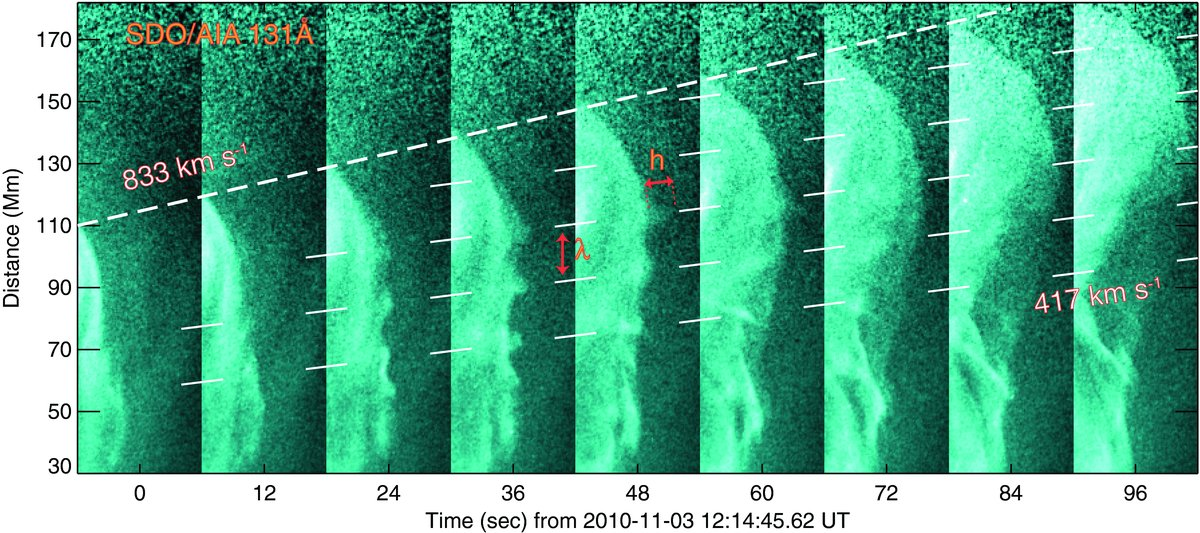
\includegraphics[width=\textwidth]{figures/khi_cme.jpg}
\caption{A time-distance plot of the KHI observed on the flank of a CME in \cite{Foullon2011}.
The parameters $\lambda$ and $h$ correspond to the distance between the KH vortices, and the maximum height of a vortex as measured from the flank, respectively.
}
\label{fig:khicme}
\end{figure}

Of particular interest in this Thesis are the observations of the KHI on the flanks of CMEs (see Figure \ref{fig:khicme}).
It was suggested by \cite{Foullon2011} and \cite{Mostl2013}, that the region on the CME flank where the instability occurs may be modelled as a thin slab in an asymmetric environment.
\cite{Mostl2013} demonstrated that by increasing the strength of the magnetic field on one side of the slab, the KHI on that side is inhibited.
This numerical study shows that exterior asymmetry is an important factor when considering the physics of magnetic slabs.
The observations of \cite{Ofman2011, Foullon2011, Mostl2013} are further discussed in Chapter 2.

\section{Outline of Thesis}

In this Thesis, we study the stability of two MHD configurations subjected to shear flows, and discuss their applications to solar phenomena.
In Chapter 2, we study the steady slab embedded in a static non-magnetic asymmetric environment.
Our analysis starts with the derivation of the governing equations for each section of the system, which was omitted in our discussion of a slab in a symmetric environment in Section \ref{sec:mhdwaves}.
We, then, obtain a dispersion relation for waves propagating along the slab, and some of its approximate solutions.
We solve the dispersion relation numerically to obtain general wave solutions and determine the KHI threshold.
Finally, we discuss how our model may be used for the seismology of KH unstable CMEs.

In Chapter 3, we study an interface separating time-periodic counter streaming flows.
We find that the governing equation for perturbations perpendicular to the interface is Mathieu's equation, and we study its stability.
We discuss our findings in the context of applications to the stability of transverse coronal loop oscillations.
